\documentclass{article}


\title{Labwork 2: Linear Regression}

\begin{document}

\maketitle

\setlength\parindent{0pt}

\section{Introduction}

Linear Regression: Finding a line/plane/hyperplane to represent for data. In this example, with 2 dimensional data, we can represent data by  a line in the form of y = w0*x + w1. 
Calculating value of w0 and w1:
w0 called as slope can be calculated as:

w1 called as intercept can be calculated as:

\usepackage{amsmath} 

In linear regression, the line of best fit is expressed as:

\[ y = w0x + w1 \]

The slope (\( w0 \)) of the linear regression line is calculated using the formula:

\[ w0 = \frac{\sum (x_i - \bar{x}) (y_i - \bar{y})}{\sum (x_i - \bar{x})^2} \]

The intercept (\( w1 \)) of the linear regression line is calculated using the formula:

\[ w1 = \bar{y} - m \cdot \bar{x} \]

Where:
- \( x_i \) and \( y_i \) are the values of the independent and dependent variables, respectively, for the \( i \)-th data point.
- \( \bar{x} \) and \( \bar{y} \) are the mean (average) values of \( x \) and \( y \).

The means of \( x \) and \( y \) can be calculated as follows:

\[ \bar{x} = \frac{\sum x_i}{n} \]

\[ \bar{y} = \frac{\sum y_i}{n} \]

Where \( n \) is the number of data points.


Usage: Predict unlabelled data. For this example, the prediction for unlabelled data can be calculate as y_prediction = w0*x_input + w1
 

\section{Implementation}

- Read data from data.csv
- Assign value for x and y respectively
- Calculate the mean for x and y
- Find w0 and w1 following above formulas. With w0, we need to calculate by y_deviation*x_deviation / x_deviation^2, and w1 = mean_y - w0 * mean_x
- After we have w0 and w1, we write a function for prediction with input is w0,w1 and x input, the output is prediction from the line 
- Finally, we need to plot data points and linear regression line for visualization


\section{Evaluation}
Test with: 
x_input =  1714,1972,1620,1000
y_output = 3.12,2.54,2.95,1.93

Linear Regression as a line and data points are showed below:
\usepackage{graphicx}
\begin{figure}[h]
    \centering
    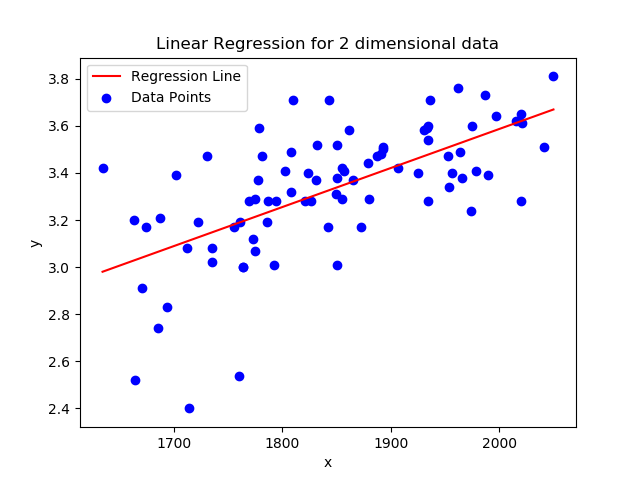
\includegraphics[width=<width>,height=<height>]{</home/noopi/dl2024/Figure_1.png>}
    \caption{<Caption text>}
    \label{<figure_label>}
\end{figure}
 

\section{Conclusion}

In this labwork, we did this, that, and the result is this.

An interesting finding is that.....

\end{document}
